\documentclass[12pt]{report} % Increased the font size to 12pt
\usepackage{epigraph}
\usepackage{geometry}

% Optional: customize the style of epigraphs
\setlength{\epigraphwidth}{0.5\textwidth} % Adjust the width of the epigraph
\renewcommand{\epigraphflush}{flushright} % Align the epigraph to the right
\renewcommand{\epigraphrule}{0pt} % No horizontal rule
\usepackage[most]{tcolorbox}
\usepackage{amsmath, amssymb, amsthm}
\usepackage{bbm}
\usepackage{graphicx}
\usepackage{caption}
\usepackage[utf8]{inputenc}
\usepackage{hyperref} % Added for hyperlinks
\usepackage{listings} % Added for code listings
\usepackage{color}    % Added for color definitions
\usepackage[super]{nth}
\usepackage{fancyhdr}
\usepackage{tikz}
\usepackage{cite}
\usetikzlibrary{shapes.geometric, arrows, positioning}

\tikzstyle{startstop} = [rectangle, rounded corners, minimum width=3cm, minimum height=1cm, text centered, draw=black, fill=red!30]
\tikzstyle{io} = [trapezium, trapezium left angle=70, trapezium right angle=110, minimum width=3cm, minimum height=1cm, text centered, draw=black, fill=blue!30]
\tikzstyle{process} = [rectangle, minimum width=3cm, minimum height=1cm, text centered, draw=black, fill=orange!30]
\tikzstyle{decision} = [diamond, minimum width=3cm, minimum height=1cm, text centered, draw=black, fill=green!30]
\tikzstyle{arrow} = [thick,->,>=stealth]

% Define the graphics path
%\graphicspath{{./Plots/}}

% Define the header and footer for general pages
\pagestyle{fancy}
\fancyhf{} % Clear all header and footer fields
\fancyhead{} % Initially, the header is empty
\fancyfoot[C]{\thepage} % Page number at the center of the footer
\renewcommand{\headrulewidth}{0pt} % No header line on the first page of chapters
\renewcommand{\footrulewidth}{0pt} % No footer line

% Define the plain page style for chapter starting pages
\fancypagestyle{plain}{%
  \fancyhf{} % Clear all header and footer fields
  \fancyfoot[C]{\thepage} % Page number at the center of the footer
  \renewcommand{\headrulewidth}{0pt} % No header line
}

% Apply the 'fancy' style to subsequent pages in a chapter
\renewcommand{\chaptermark}[1]{%
  \markboth{\MakeUppercase{#1}}{}%
}

% Redefine the 'plain' style for the first page of chapters
\fancypagestyle{plain}{%
  \fancyhf{}%
  \fancyfoot[C]{\thepage}%
  \renewcommand{\headrulewidth}{0pt}%
}

% Header settings for normal pages (not the first page of a chapter)
\fancyhead[L]{\slshape \nouppercase{\leftmark}} % Chapter title in the header
\renewcommand{\headrulewidth}{0.4pt} % Header line width on normal pages

\setlength{\headheight}{14.49998pt}
\addtolength{\topmargin}{-2.49998pt}
% Define colors for code listings
\definecolor{codegreen}{rgb}{0,0.6,0}
\definecolor{codegray}{rgb}{0.5,0.5,0.5}
\definecolor{codepurple}{rgb}{0.58,0,0.82}
\definecolor{backcolour}{rgb}{0.95,0.95,0.92}

% Setup for code listings
\lstdefinestyle{mystyle}{
    backgroundcolor=\color{backcolour},
    commentstyle=\color{codegreen},
    keywordstyle=\color{magenta},
    numberstyle=\tiny\color{codegray},
    stringstyle=\color{codepurple},
    basicstyle=\ttfamily\footnotesize,
    breakatwhitespace=false,
    breaklines=true,
    captionpos=b,
    keepspaces=true,
    numbers=left,
    numbersep=5pt,
    showspaces=false,
    showstringspaces=false,
    showtabs=false,
    tabsize=2
}

\lstset{style=mystyle}

% Definition of the tcolorbox for definitions
\newtcolorbox{definitionbox}{
  colback=red!5!white,
  colframe=red!75!black,
  colbacktitle=red!85!black,
  title=Definition:,
  fonttitle=\bfseries,
  enhanced,
}

% Definition of the tcolorbox for remarks
\newtcolorbox{remarkbox}{
  colback=blue!5!white,     % Light blue background
  colframe=blue!75!black,   % Darker blue frame
  colbacktitle=blue!85!black, % Even darker blue for the title background
  title=Remark:,            % Title text for remark box
  fonttitle=\bfseries,      % Bold title font
  enhanced,
}

% Definition of the tcolorbox for examples
\newtcolorbox{examplebox}{
  colback=green!5!white,
  colframe=green!75!black,
  colbacktitle=green!85!black,
  title=Example:,
  fonttitle=\bfseries,
  enhanced,
}

% Definitions and examples will be put in these environments
\newenvironment{definition}
    {\begin{definitionbox}}
    {\end{definitionbox}}

\newenvironment{example}
    {\begin{examplebox}}
    {\end{examplebox}}

\geometry{top=1.5in} % Adjust the value as needed
% ----------------------------------------------------------------------------------------


\title{S2 Statistics for Data Science}
\author{CRSiD: tmb76}
\date{University of Cambridge}

\begin{document}

\maketitle

\tableofcontents

\chapter*{The Lighthouse Problem}

\section*{The Setup}

\indent A lighthouse that is at a distance $\beta$ from the coast is at position $\alpha$ along it. The lighthouse emits flashes at random angles $\theta$, following a uniform distribution. The flashes can be considered narrow and, provided $\pi/2 < \theta < \pi/2$, intersect the coastline at a single point. Detectors on the coastline record only the flashes' locations $x_{k}$ (where $k = 1, 2,\dots, N$ ) for N flashes received. The setup is illustrated in Figure \ref{fig:lighthouse}.

\begin{figure}[h]
\centering
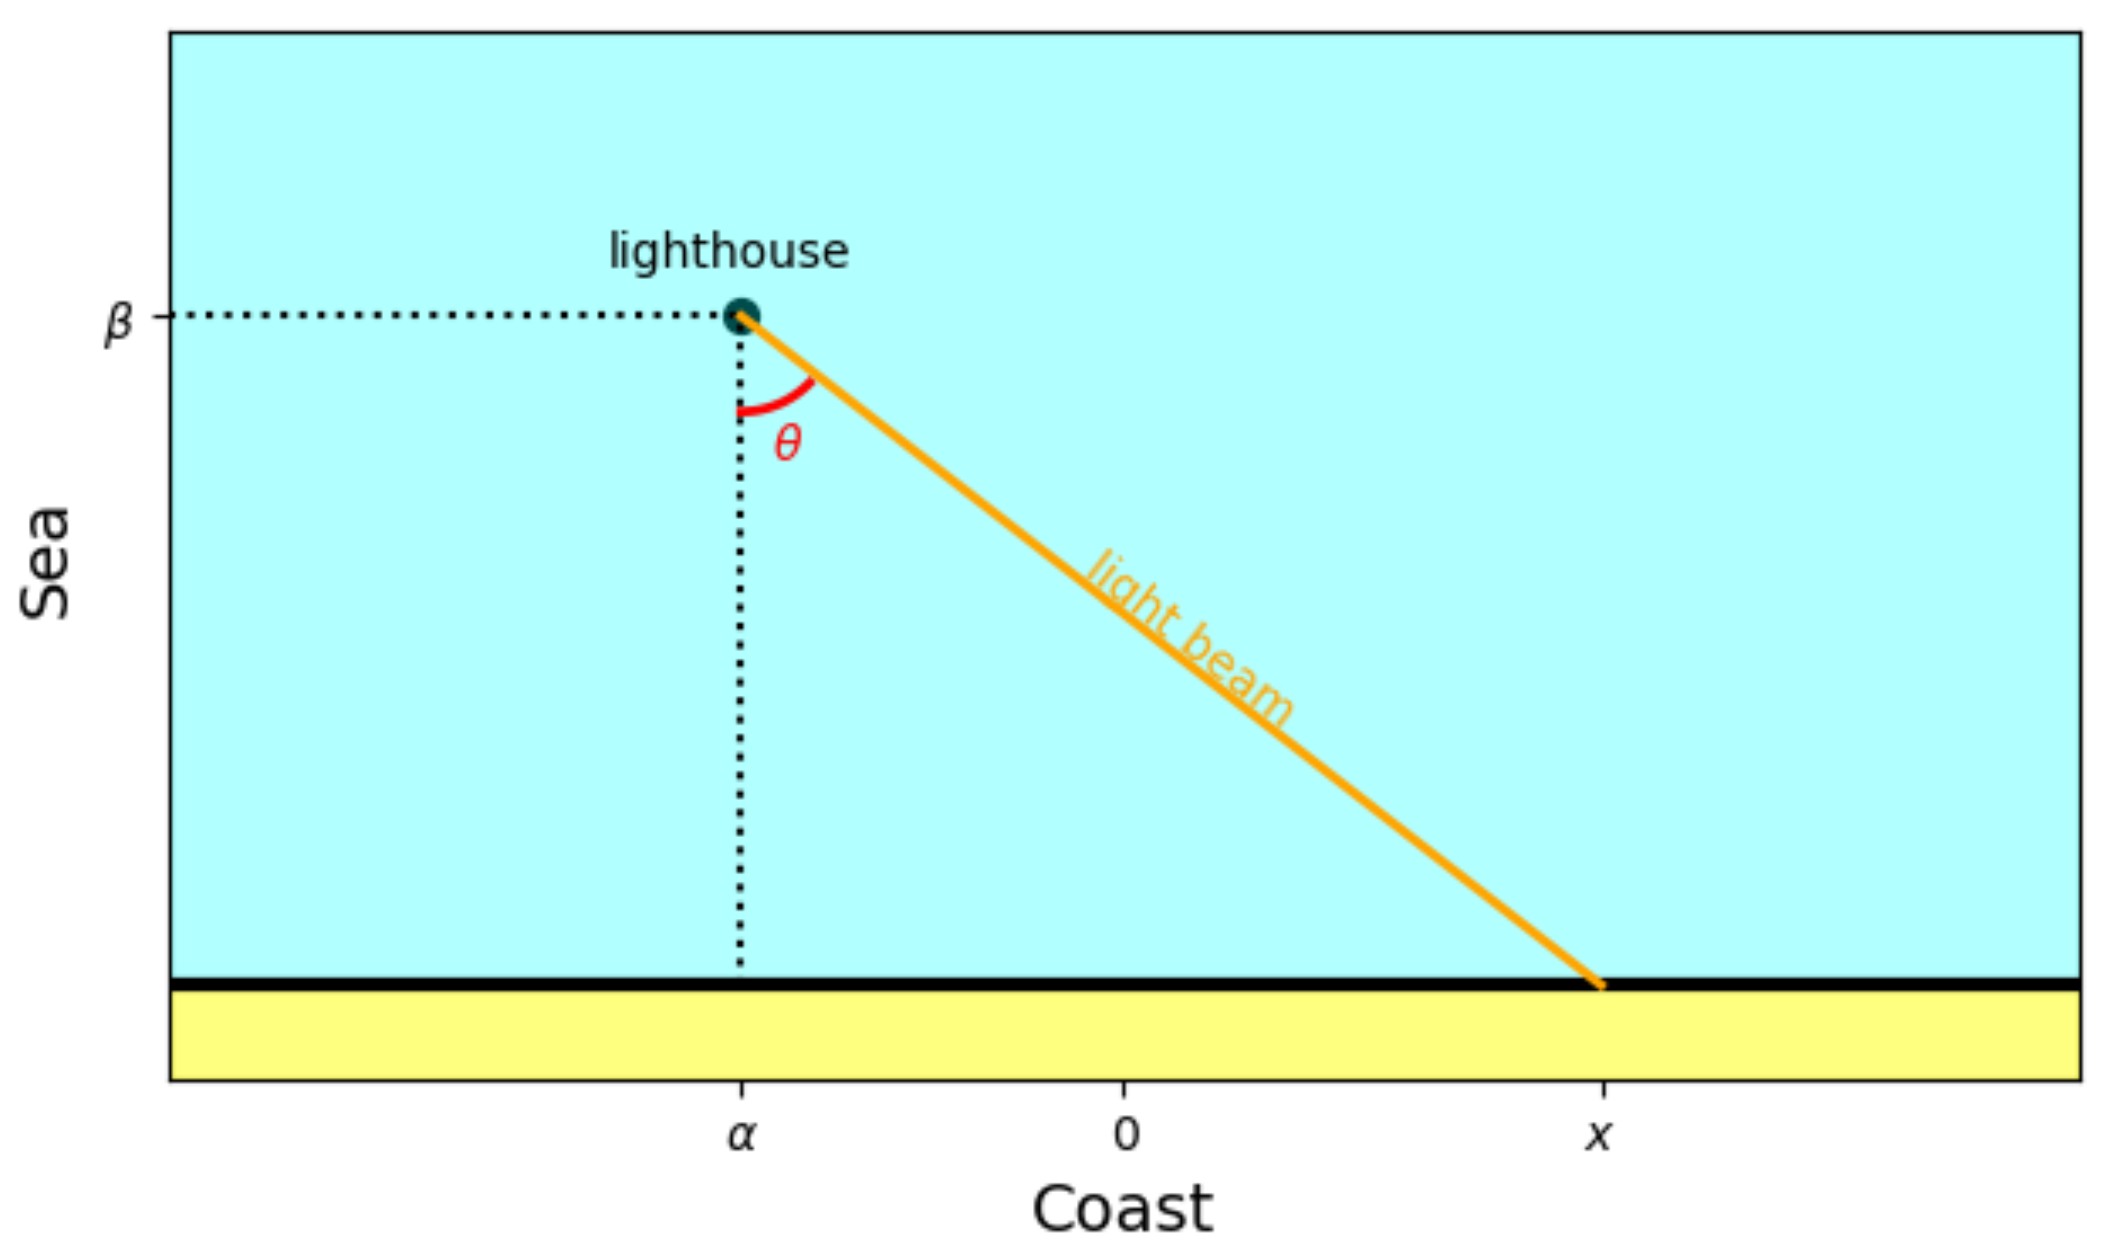
\includegraphics[width=0.8\textwidth]{../Plots/lighthouse diagram.png}
\caption{The lighthouse problem setup}
\label{fig:lighthouse}
\end{figure}


The goal of this project is to find the location of the lighthouse from the recorded data ${x_{k}}$.

\subsection*{(i) The Geometry of the Problem}

As stated above, only the distribution of the flashes' angle, $\theta$, is known. However, the observed data obtained is the location of the flashes on the coastline, $x_{k}$. Thus, it is worth considering what the relationship is between the angle of the flash and the location of the flash on the coastline, expressed in terms of the unknown lightouse location parameters $\alpha$ and $\beta$. Using trigonometry, the following relationship can be derived:

\begin{equation}
    x = \alpha + \beta \tan(\theta) \iff \theta = \tan^{-1}\left(\frac{x - \alpha}{\beta}\right)
\end{equation}

\subsection*{(ii) The Likelihood Function}

In addition to the relationship above, the probability distribution of the flashes' angles is known to be uniform. Thus, the probability of a single flash to have the angle $\theta$ is given by:

\begin{equation}
    \theta \sim U(-\pi/2, \pi/2)
\end{equation}

\begin{equation}
    P(\theta) = \mathbbm{1}_{(-\pi/2, \pi/2)}(\theta) \times \frac{1}{\pi} = \begin{cases} \frac{1}{\pi}, & \text{if } -\frac{\pi}{2} < \theta < \frac{\pi}{2} \\ 0, & \text{otherwise} \end{cases}
\end{equation}

Now, using the trigonometric relationship between $\theta$ and $x$ derived in (1), a change of variable is conducted to find the probability distribution of the flashes' locations on the coastline, $x$. Here, this will be considered as the likelihood of a single flash to be observed at location $x$ given the lighthouse location parameters $\alpha$ and $\beta$. For this 1-D case, the change of variable can be written as:

\begin{equation}
    \mathcal{L}_{x}(x|\alpha, \beta) = \mathcal{L}_{\theta}(\theta) \times \left| \frac{d\theta}{dx} \right|
\end{equation}

$\mathcal{L}_{\theta}(\theta)$ is the probability distribution of the flashes' angles, which is given in Equation (3). Since the angle $\theta$ must be such that $-\pi/2 < \theta < \pi/2$ for the flash to be observed on the coastline, $\mathcal{L}_{\theta}(\theta)$ can be set to $1/\pi$. The dereivative term is given by:

\begin{equation}
    \frac{d\theta}{dx} = \frac{d}{dx} (\tan^{-1}\left(\frac{x - \alpha}{\beta}\right) )
\end{equation}

Using the chain rule, the derivative can be found to be:

\begin{equation}
    \frac{d\theta}{dx} = \frac{1}{1 + \left(\frac{x - \alpha}{\beta}\right)^{2}} \times \frac{1}{\beta}
\end{equation}

With some algebraic manipulation, this can be re-arranged as:

\begin{equation}
    \frac{d\theta}{dx} = \frac{\beta}{\beta^{2} + (x - \alpha)^{2}}
\end{equation}

Thus the likelihood for a single flash to be observed at location $x$ given the lighthouse location parameters $\alpha$ and $\beta$ is:

\begin{equation}
    \mathcal{L}_{x}(x|\alpha, \beta) = \frac{1}{\pi} \times \frac{\beta}{\beta^{2} + (x - \alpha)^{2}}
\end{equation}

as required.

\subsection*{(iii) Frequentist Claim}

A frequentist colleague claims the most likely location, $\hat{x}$, for any flash to be received is given by the parameter $\alpha$, the location of the lighthouse along the coastline. They also suggest using the sample mean to estimate the $\alpha$ parameter. This turns out to be a bad estimator. First, the $hat{x} = \alpha$ claim. $hat_{x}$ is the location for which the likelihood in Eq. (8) is maximised. This is found by taking the derivative of the likelihood with respect to $x$ and setting it to zero. This gives:

\begin{equation}
    \left. \frac{d\mathcal{L}_{x}(x|\alpha, \beta)}{dx} \right|_{x = \hat{x}} = 0 \iff \left. \frac{d}{dx} \left(\frac{\beta}{\beta^{2} + (x - \alpha)^{2}}\right) \right|_{x = \hat{x}} = 0
\end{equation}

\begin{equation}
    -\frac{1}{\pi} \beta (2\hat{x} - 2\alpha)\frac{1}{\beta^{4} + 2\beta^{2}(\hat{x} - \alpha)^{2} + (\hat{x} - \alpha)^{4}} =
\end{equation}
\newline
This is satisfied when $\hat{x} = \alpha$, as claimed. Thus, the frequentist's claim is accurate for the value of the most likely flash location. However, estimating the value of $\alpha$ with the sample mean is not good. To show this, we compare it with the Maximum Likelihood Estimate (MLE) method. The aim is to find the value of $\alpha$ that maximises the likelihood derived in Eq. (8), based on the observed sample ${x_k}$ ($k = 1, 2,\dots, N$). This means now having the likelihood being the product of individula likelihoods for all values of ${x_k}$. This is done by taking the derivative of the likelihood with respect to $\alpha$ and setting it to zero. However, for simplicity in derivation and computation, the log-likelihood is used instead.

\begin{equation}
    \hat{\alpha}_{MLE} = \arg \max_{\alpha} \ln(\prod_{k=1}^{N}  \mathcal{L}_{x}(x_{k}|\alpha, \beta)) = \arg \max_{\alpha} \sum_{k=1}^{N} \ln(\frac{1}{\pi} \times \frac{\beta}{\beta^{2} + (x_{k} - \alpha)^{2}})
\end{equation}

\begin{equation}
    \hat{\alpha}_{MLE} = \arg \max_{\alpha} \sum_{k=1}^{N} \ln(\frac{\beta}{\pi}) + \ln(\frac{1}{(\beta^{2} + (x_{k} - \alpha)^{2})})
\end{equation}

\begin{equation}
    \left. \frac{d}{d\alpha} \left( \sum_{k=1}^{N} \ln(\frac{\beta}{\pi}) + \ln(\frac{1}{(\beta^{2} + (x_{k} - \alpha)^{2})}) \right) \right|_{\alpha = \hat{\alpha}_{MLE}} = 0
\end{equation}

\begin{equation}
    \sum_{k=1}^{N} \left. \frac{(2\alpha - 2x_{k})}{(\beta^{2} + (x_{k} - \alpha)^{2})} \right|_{\alpha = \hat{\alpha}_{MLE}} = 0
\end{equation}
\newline
To get an estimate of $\hat{\alpha}_{MLE}$, the above equation needs to be rearranged to isolate $\alpha$. However, this is difficult to do analytically. More importantly, the overarching issue is that the Cauchy distribution does not follow the Central Limit Theorem. This is shown in the fact that the distribution of the sample mean of the Cauchy distribution is itself a Cauchy distribution, no matter the sample size:



\subsection*{(iv) Priors for $\alpha$ and $\beta$}

Uniform for $\alpha$ and $\beta$. cuz it makes sense.

\subsection*{(v) Stochastic Sampling }




\end{document}
